\documentclass{math}

\usepackage{graphicx}
\usepackage{listings}

\title{Principles of Data Mining: HW 02}
\author{Alvin Lin}
\date{August 2018 - December 2018}
\begin{document}

\maketitle

\subsubsection*{Question 1a}
To maximize public safety, we would want to use a lower speed threshold in the
event of a tie to catch more speeders. This would result in more true positives
at the cost of also increasing false positives. Since we want to maximize
public safety, we are more concerned with maximizing true positives.

\subsubsection*{Question 1b}
To maximize public trust, we would want to use a higher speed threshold in the
event of a tie to reduce the number of false positives. This would result in
more false negatives since we would be letting by more speeders who intended to
speed and/or are driving recklessly. Since we want to maximize public trust, we
are more concerned with minimizing false positives.

\subsubsection*{Question 1d}
\begin{center}
  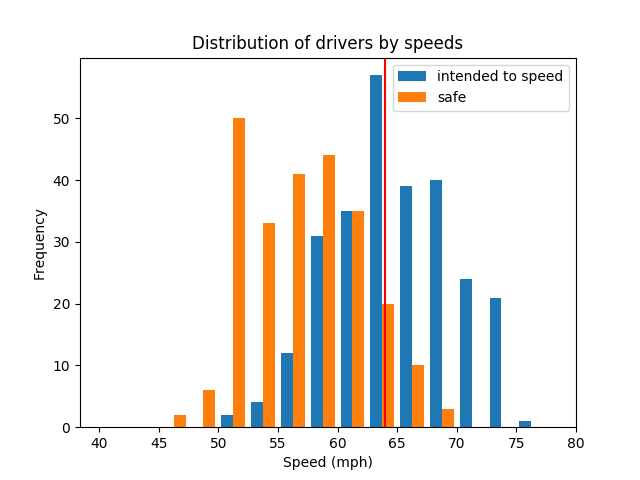
\includegraphics[width=16cm]{assets/hw_02_speed_histogram.png}
\end{center}
Using a cost function that penalizes false positives, I computed a threshold of
64 miles per hour. Using a cost function that penalizes false negatives instead,
I computed a threshold of 56 miles per hour. The diagram above marks the first
threshold in red.

\subsubsection*{Question 1e}
For this given training data, there were 114 false negatives, meaning 114
reckless drivers were let through. This corresponds to a 3.51\% false negative
rate.

\subsubsection*{Question 1f}
For this given training data, there were 18 false positives, meaning 18
non-reckless drivers were pulled over. This corresponds to a 22.27\% false
positive rate.

\subsubsection*{Question 1g}
Using Otsu's method, a threshold of 61 miles per hour was computed, which had
a 54 false positives and 68 false negatives (10.5\% and 13.3\% respectively).
Otsu's method does not take into account the false negative or false positive
rate when computing its threshold.

\subsubsection*{Question 1h}
\begin{center}
  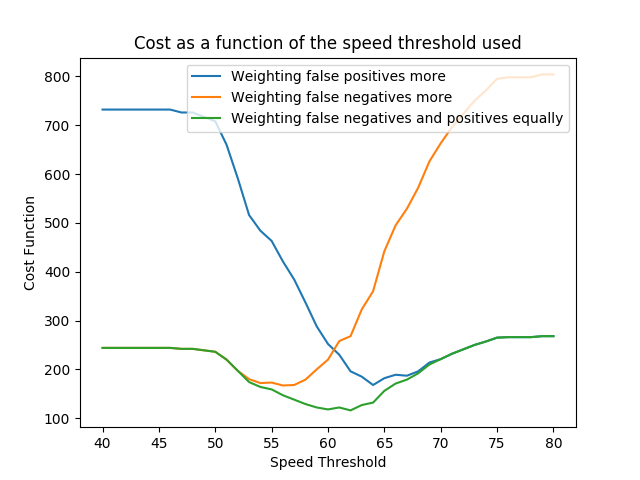
\includegraphics[width=16cm]{assets/hw_02_cost_vs_threshold.png}
\end{center}

\subsubsection*{Question 1i}
Depending on what the objective is, a different speed threshold should be
chosen. In the interest of maximizing public safety, a speed threshold of
64 miles per hour should be chosen in order to minimize false negatives, which
would result in less reckless drivers getting away. In the interest of
maximizing public trust, a lower speed threshold of 56 miles per hour should be
used to minimize false positives, and thus reduce the amount of non-reckless
drivers pulled over. Realistically, a higher speed threshold should be used
because even if people don't intend to speed, they are endangering other people
by driving at a high speed. \par
These classification methods could be applied to multi dimensional data if the
data can be grouped and classified by a feature in one dimension. This would
help us reveal if the other dimensions are dependent on any one dimension. It
would help us find correlations between the dimensions. \par
While nothing was particularly difficult, this was a good exercise in using the
powerful features that \texttt{numpy} provides. In particular, \texttt{numpy}'s
powerful array indexing features and syntactic sugar allow for certain things to
be done very quickly and easily. The only downside to syntactic sugar is that
the code can become very convoluted to someone who is not familiar with
\texttt{numpy}.

\subsubsection*{Question 2 (Bonus)}
\begin{center}
  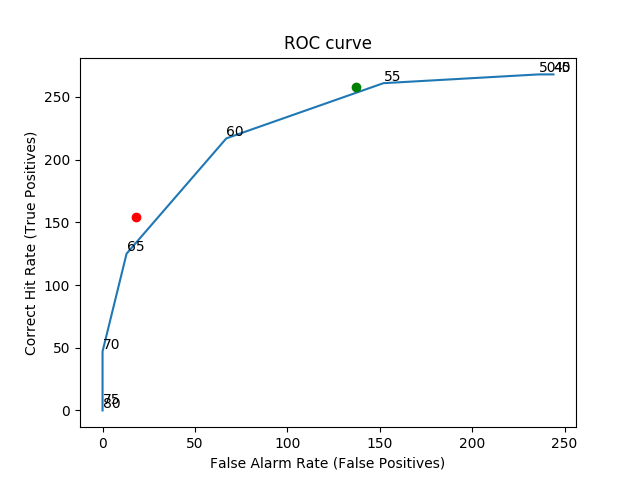
\includegraphics[width=16cm]{assets/hw_02_roc_curve.png}
\end{center}
The red point represents a threshold of 64, and has the lowest cost when
penalizing false positives. The green point represents a threshold of 56,
and has the lowest cost when penalizing false negatives.

\begin{center}
  If you have any questions, comments, or concerns, please contact me at
  alvin@omgimanerd.tech
\end{center}

\end{document}
